\documentclass{article}
\usepackage{tikz}
\usepackage{amsmath, amssymb}
\usetikzlibrary{calc}
\usepgflibrary{fpu}
\begin{document}

\begin{enumerate}

	\item Draw the following vectors in standard position in R$^{2}$

	\begin{enumerate}

	\item $\text{a } = \begin{bmatrix} 3 \\ 0 \\ \end{bmatrix} $

	\item $\text{b } = \begin{bmatrix} 2 \\ 3 \\ \end{bmatrix} $

	\item $\text{c } = \begin{bmatrix} -2 \\ 3 \\ \end{bmatrix}$

	\item $\text{d } = \begin{bmatrix} 3 \\ -2 \\ \end{bmatrix}$

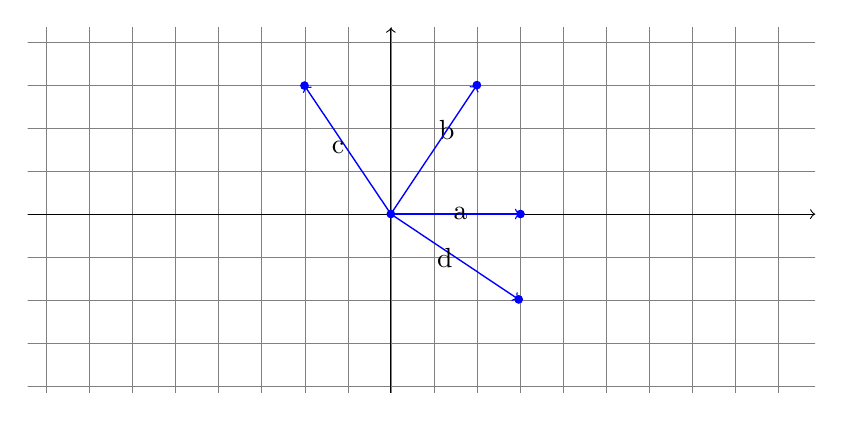
\begin{tikzpicture}[%
scale=0.546427,
]
\clip (-8.44094,-4.15788) rectangle (9.85978,4.33184);
\draw [help lines] (0,0) grid (10,5);
\draw [help lines] (-9,0) grid (0,5);
\draw [help lines] (0,-5) grid (10,0);
\draw [help lines] (-9,-5) grid (0,0);
\draw [color=black,->] (-8.44094,0) -- (9.85978,0);
\draw [color=black,->] (0,-4.15788) -- (0,4.33184);
%% point;
\filldraw [color={rgb:red,0;green,0;blue,255}] (1.99927,2.99627) circle (2.5pt );
%% vector;
\draw[color={rgb:red,0;green,0;blue,255}, line width=0.5pt, solid, ->] (0,0.000547801) -- (3.01218,0.000547801);
%% point;
\filldraw [color={rgb:red,0;green,0;blue,255}] (2.97045,-1.98382) circle (2.5pt );
%% point;
\filldraw [color={rgb:red,0;green,0;blue,255}] (0,0.000547801) circle (2.5pt );
%% vector;
\draw[color={rgb:red,0;green,0;blue,255}, line width=0.5pt, solid, ->] (0,0.000547801) -- (-2.00686,2.98488);
%% point;
\filldraw [color={rgb:red,0;green,0;blue,255}] (-2.00686,2.98488) circle (2.5pt );
%% label;
\node at (1.61303,0.000547801) {a};
%% point;
\filldraw [color={rgb:red,0;green,0;blue,255}] (3.01218,0.000547801) circle (2.5pt );
%% label;
\node at (1.30014,1.94869) {b};
%% vector;
\draw[color={rgb:red,0;green,0;blue,255}, line width=0.5pt, solid, ->] (0,0.000547801) -- (2.97045,-1.98382);
%% label;
\node at (1.25574,-1.02064) {d};
%% vector;
\draw[color={rgb:red,0;green,0;blue,255}, line width=0.5pt, solid, ->] (0,0.000547801) -- (1.99927,2.99627);
%% label;
\node at (-1.22843,1.55652) {c};
\end{tikzpicture}

	\end{enumerate}

	\item Draw the vectors in Exercise 1 with their tails at the
		point (1, -3).

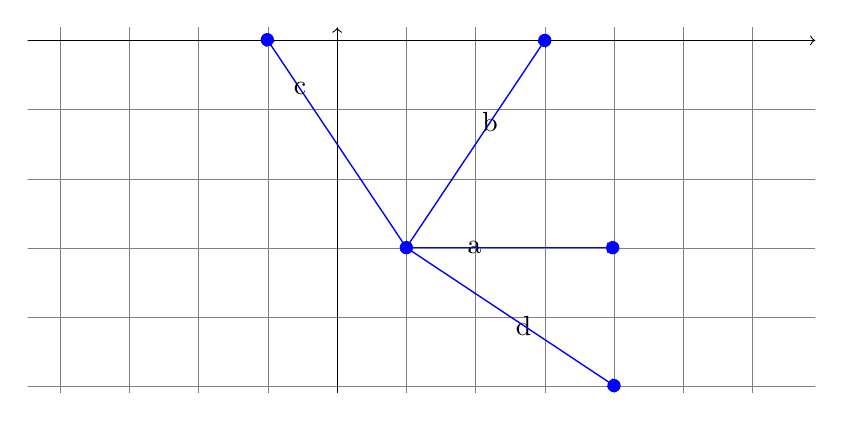
\begin{tikzpicture}[%
scale=0.879603,
]
\clip (-4.46832,-5.09049) rectangle (6.90044,0.183483);
\draw [help lines] (0,0) grid (7,1);
\draw [help lines] (-5,0) grid (0,1);
\draw [help lines] (0,-6) grid (7,0);
\draw [help lines] (-5,-6) grid (0,0);
\draw [color=black,->] (-4.46832,0) -- (6.90044,0);
\draw [color=black,->] (0,-5.09049) -- (0,0.183483);
%% label;
\node at (1.97963,-2.99268) {a};
%% point;
\filldraw [color={rgb:red,0;green,0;blue,255}] (0.999244,-2.99268) circle (2.5pt );
%% vector;
\draw[color={rgb:red,0;green,0;blue,255}, line width=0.5pt, solid, ->] (0.999244,-2.99268) -- (2.99773,-8.88178e-4);
%% vector;
\draw[color={rgb:red,0;green,0;blue,255}, line width=0.5pt, solid, ->] (0.999244,-2.99268) -- (3.97812,-2.99268);
%% point;
\filldraw [color={rgb:red,0;green,0;blue,255}] (3.97812,-2.99268) circle (2.5pt );
%% label;
\node at (2.6903,-4.11616) {d};
%% vector;
\draw[color={rgb:red,0;green,0;blue,255}, line width=0.5pt, solid, ->] (0.999244,-2.99268) -- (-1.00867,0.00942683);
%% point;
\filldraw [color={rgb:red,0;green,0;blue,255}] (2.99773,-8.88178e-4) circle (2.5pt );
%% label;
\node at (2.20786,-1.18281) {b};
%% point;
\filldraw [color={rgb:red,0;green,0;blue,255}] (-1.00867,0.00942683) circle (2.5pt );
%% vector;
\draw[color={rgb:red,0;green,0;blue,255}, line width=0.5pt, solid, ->] (0.999244,-2.99268) -- (3.99698,-4.98427);
%% point;
\filldraw [color={rgb:red,0;green,0;blue,255}] (3.99698,-4.98427) circle (2.5pt );
%% label;
\node at (-0.537741,-0.694678) {c};
\end{tikzpicture}

	\item Draw the following vectors in standard position in R$^{3}$.

	\begin{enumerate}
		\item $\text{a } = \begin{bmatrix} 0, & 2, & 1 \end{bmatrix}$

		\item $\text{b } = \begin{bmatrix} 3, & 2, & 1 \end{bmatrix}$

		\item $\text{c } = \begin{bmatrix} 1, & -2, 1 \end{bmatrix}$

		\item $\text{d } = \begin{bmatrix} -1, & -1, & -2 \end{bmatrix}$
	\end{enumerate}

	\item If the vectors in Exercise 3 are translated so that their
		heads are at the point $(1, 2, 3)$, find the points that
		correspond to their tails.

	\begin{enumerate}

		\item $\text{a } = (1,0,2)$

		\item $\text{b } = (-2,0,2)$

		\item $\text{c } = (0,4,2)$

		\item $\text{d } = (2,3,5)$

	\end{enumerate}

\end{enumerate}
\end{document}
